\documentclass{ceri}
\title{Preliminary Design Alternatives Report}
\usepackage[final]{pdfpages}
\usepackage[driver=pdftex]{geometry}
\addbibresource{bibliographie.bib}
\usepackage{longtable}
\usepackage[colorlinks=true]{hyperref}
\tolerance=1
\emergencystretch=\maxdimen
\hyphenpenalty=10000
\hbadness=10000
\widowpenalty10000
\clubpenalty10000
\newcommand{\myparagraph}[1]{\paragraph{#1}\mbox{}\\}
\usepackage{etoolbox,refcount}
\usepackage{multicol}
\usepackage{graphicx}
\usepackage{booktabs}
\usepackage{lscape}
\usepackage[table,xcdraw]{xcolor}
\newcounter{countitems}
\newcounter{nextitemizecount}
\newcommand{\setupcountitems}{%
  \stepcounter{nextitemizecount}%
  \setcounter{countitems}{0}%
  \preto\item{\stepcounter{countitems}}%
}
\makeatletter
\newcommand{\computecountitems}{%
  \edef\@currentlabel{\number\c@countitems}%
  \label{countitems@\number\numexpr\value{nextitemizecount}-1\relax}%
}
\newcommand{\nextitemizecount}{%
  \getrefnumber{countitems@\number\c@nextitemizecount}%
}
\newcommand{\previtemizecount}{%
  \getrefnumber{countitems@\number\numexpr\value{nextitemizecount}-1\relax}%
}
\makeatother    
\newenvironment{AutoMultiColItemize}{%
\ifnumcomp{\nextitemizecount}{>}{3}{\begin{multicols}{2}}{}%
\setupcountitems\begin{itemize}}%
{\end{itemize}%
\unskip\computecountitems\ifnumcomp{\previtemizecount}{>}{3}{\end{multicols}}{}}
\newcommand{\namesigdate}[2][5cm]{%
  \begin{tabular}{@{}p{#1}@{}}
    #2 \\[2\normalbaselineskip] \hrule \\[0pt]
    {\small \textit{Signature}} \\[2\normalbaselineskip] \hrule \\[0pt]
    {\small \textit{Printed Name}}\\[2\normalbaselineskip] \hrule \\[0pt]
    {\small \textit{Title}}\\[2\normalbaselineskip] \hrule \\[0pt]
    {\small \textit{Date}}
  \end{tabular}
}

\begin{document} 
\maketitle
\sloppy     
\pagenumbering{arabic}
\section{Cover Letter}
\setlength{\parindent}{0pt}
February 4, 2019
\newline

\newpage
\setlength{\parindent}{8pt}
\section{Executive Summary}
Text Here:

\section{Project Understanding}

\subsection{Purpose}
Text Here:

\subsection{Project Summary}
Text Here:

\newpage
\subsection{Site Location}
The proposed project site will be located roughly five miles southwest of downtown Memphis, Tennessee inside the Frank C. Pidgeon Industrial Park. \textbf{Figure \ref{fig:Location}} depicts the proposed project site boundaries and location. 
\begin{figure}[H]
    \centering
    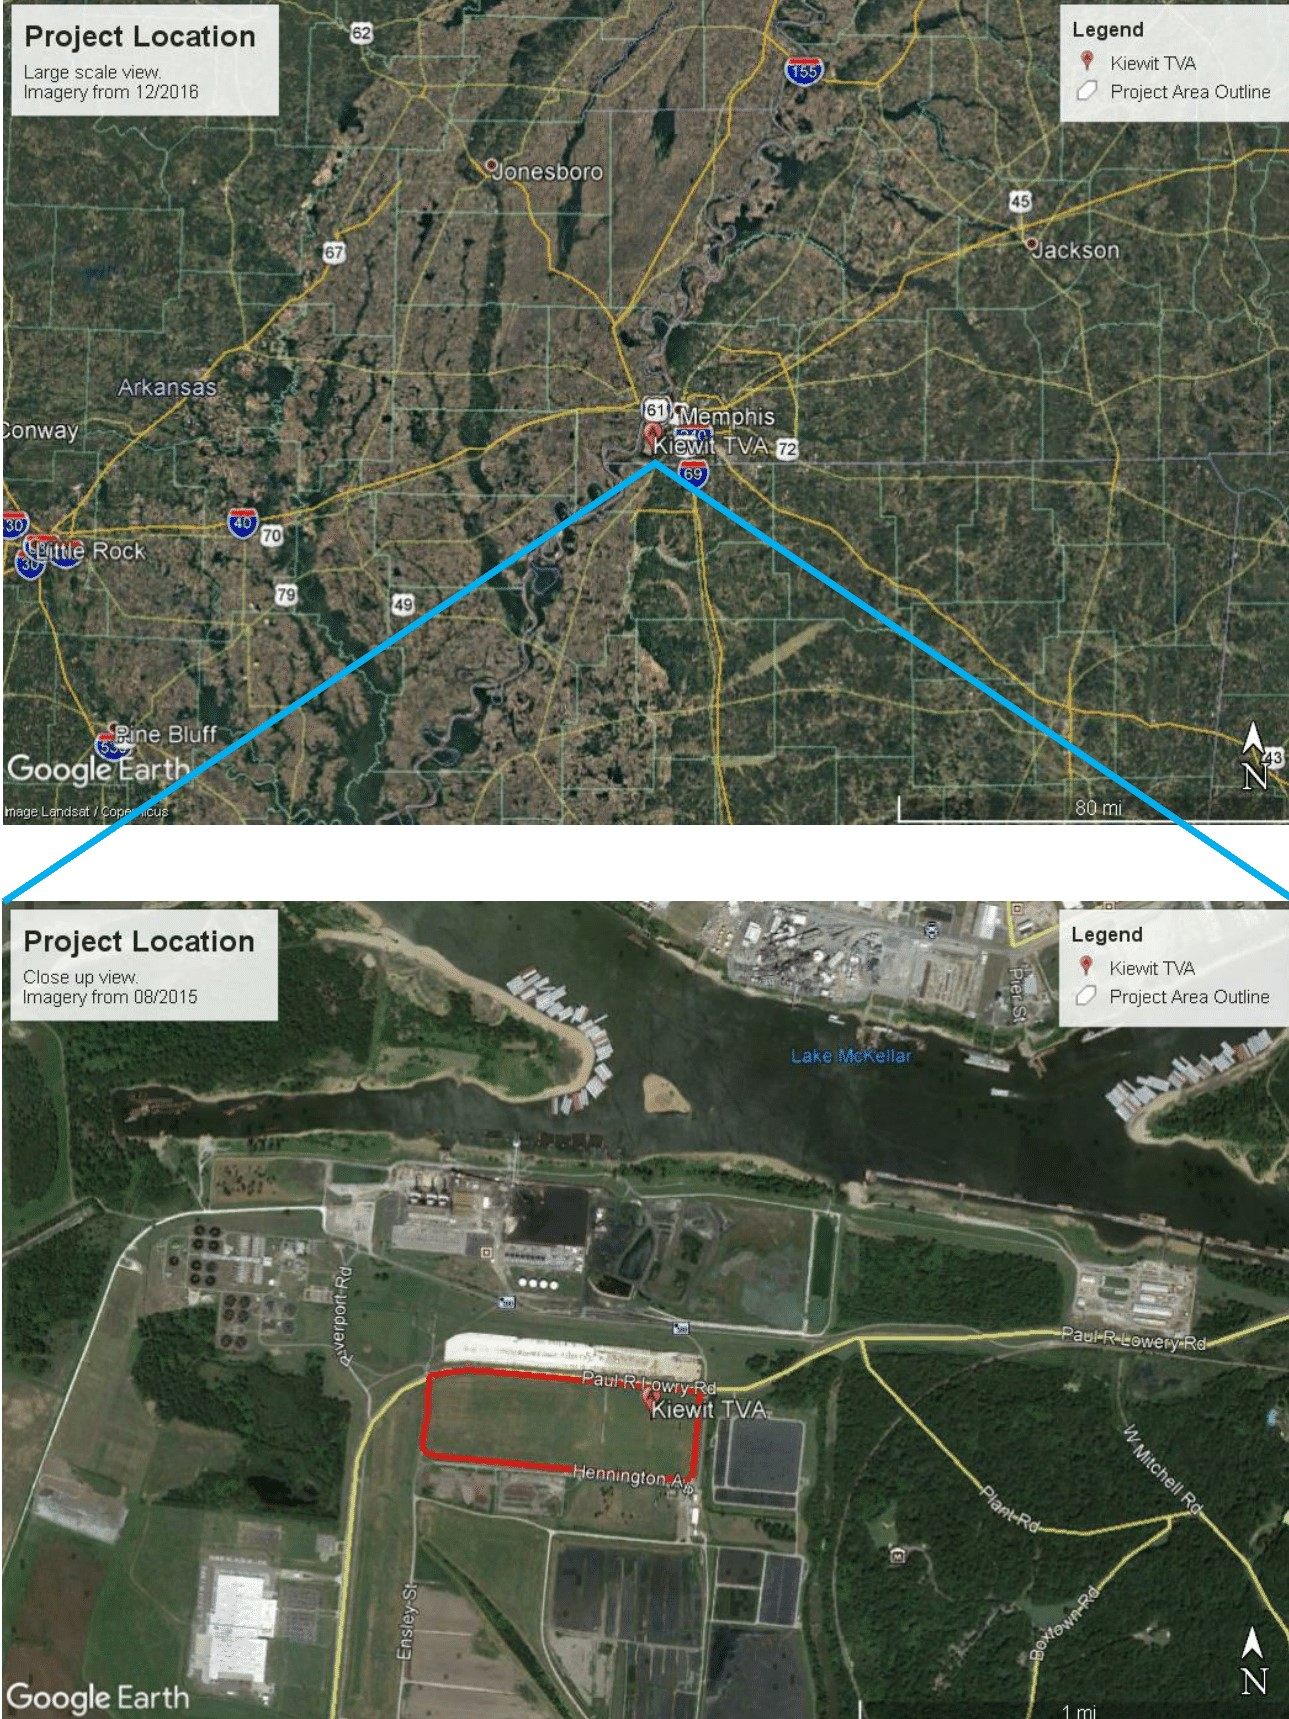
\includegraphics[width=.8\textwidth]{images/Location.png}
    \caption{Aerial View of Project Site}
    \label{fig:Location}
\end{figure}
\section{Engineers scope of Work}
Text Here:

\subsection{Civil Engineering}
Text Here:

\subsection{Architectural Engineering}
Text Here:

\subsection{Environmental Engineering}
Text Here:

\subsection{Construction}
Text Here:

\section{Method of evaluation of alternatives}
Text Here:

\section{Alternative Design Options}
\subsection{Landscaping}
Optional Text here:

\subsubsection{Alternative 1 - Name of Alternative}
Text Here:

\subsubsection{Alternative 2 - Name of Alternative}
Text Here:

\subsubsection{Landscaping Design Decision Matrix}
Text Here:

%IGNORE ME - Dane will handle this!
\begin{table}[H]
\centering
\caption{Landscaping Design Decision Matrix}
\label{my-label}
\resizebox{\textwidth}{!} & \textbf{20\%} & \textbf{20\%} & \textbf{20\%} & \textbf{20\%} & \textbf{100\%} \\
\rowcolor[HTML]{DAE8FC} 
\textbf{Option} & \textbf{Attribute 1} & \textbf{Attribute 2} & \textbf{Attribute 3} & \textbf{Attribute 4} & \textbf{Attribute 5} & \textbf{Score} \\
\textbf{Option A} & 0 & 0 & 0 & 0 & 0 & 0 \\
\textbf{Option B} & 0 & 0 & 0 & 0 & 0 & 0 \\
\rowcolor[HTML]{9AFF99} 
\textbf{Option C} & 1 & 1 & 1 & 1 & 1 & 1 \\
\textbf{Option D} & 0 & 0 & 0 & 0 & 0 & 0
\end{tabular}%
}
\end{table}
%IGNORE ME - Dane will handle this!

\subsubsection{Landscaping Design Conclusions and Recommendations}
Text Here:
\subsection{Drainage Routing}
Optional Text Here:

\subsubsection{Alternative 1 - Name of Alternative}
Text Here:

%Location Picture here

\subsubsection{Alternative 2 - Name of Alternative}
Text Here:

\subsubsection{Drainage Design Decision Matrix}
Text Here:

%IGNORE ME - Dane will edit this!
\begin{table}[H]
\centering
\caption{Drainage Design Decision Matrix}
\label{my-label}
\resizebox{\textwidth}{!} & \textbf{20\%} & \textbf{20\%} & \textbf{20\%} & \textbf{20\%} & \textbf{100\%} \\
\rowcolor[HTML]{DAE8FC} 
\textbf{Option} & \textbf{Attribute 1} & \textbf{Attribute 2} & \textbf{Attribute 3} & \textbf{Attribute 4} & \textbf{Attribute 5} & \textbf{Score} \\
\textbf{Option A} & 0 & 0 & 0 & 0 & 0 & 0 \\
\textbf{Option B} & 0 & 0 & 0 & 0 & 0 & 0 \\
\rowcolor[HTML]{9AFF99} 
\textbf{Option C} & 1 & 1 & 1 & 1 & 1 & 1 \\
\textbf{Option D} & 0 & 0 & 0 & 0 & 0 & 0
\end{tabular}%
}
\end{table}
%IGNORE ME - Dane will edit this!

\subsubsection{Drainage Design Conclusions and Recommendations}
Text Here:

\subsection{Industrial Waste Water Treatment}
Optional Text Here:

\subsubsection{Alternative 1 - Name of Alternative}
Text Here:

\subsubsection{Alternative 2 - Name of Alternative}
Text Here:

\subsubsection{Waste Water Treatment Design Decision Matrix}
Text Here:

%IGNORE ME - Dane will edit this!
\begin{table}[H]
\centering
\caption{Waste Water Treatment Design Decision Matrix}
\label{my-label}
\resizebox{\textwidth}{!} & \textbf{20\%} & \textbf{20\%} & \textbf{20\%} & \textbf{20\%} & \textbf{100\%} \\
\rowcolor[HTML]{DAE8FC} 
\textbf{Option} & \textbf{Attribute 1} & \textbf{Attribute 2} & \textbf{Attribute 3} & \textbf{Attribute 4} & \textbf{Attribute 5} & \textbf{Score} \\
\textbf{Option A} & 0 & 0 & 0 & 0 & 0 & 0 \\
\textbf{Option B} & 0 & 0 & 0 & 0 & 0 & 0 \\
\rowcolor[HTML]{9AFF99} 
\textbf{Option C} & 1 & 1 & 1 & 1 & 1 & 1 \\
\textbf{Option D} & 0 & 0 & 0 & 0 & 0 & 0
\end{tabular}%
}
\end{table}
%IGNORE ME - Dane will edit this!

\subsubsection{Waste Water Treatment Conclusions and Recommendations}
Text Here:

\subsection{Structural}
Optional Text Here:

\subsubsection{Alternative 1 - Name of Alternative}
Text Here:

\subsubsection{Alternative 2 - Name of Alternative}
Text Here:

\subsubsection{Structural Design Decision Matrix}
Text Here:

%IGNORE ME - Dane will edit this!
\begin{table}[H]
\centering
\caption{Structural Design Decision Matrix}
\label{my-label}
\resizebox{\textwidth}{!} & \textbf{20\%} & \textbf{20\%} & \textbf{20\%} & \textbf{20\%} & \textbf{100\%} \\
\rowcolor[HTML]{DAE8FC} 
\textbf{Option} & \textbf{Attribute 1} & \textbf{Attribute 2} & \textbf{Attribute 3} & \textbf{Attribute 4} & \textbf{Attribute 5} & \textbf{Score} \\
\textbf{Option A} & 0 & 0 & 0 & 0 & 0 & 0 \\
\textbf{Option B} & 0 & 0 & 0 & 0 & 0 & 0 \\
\rowcolor[HTML]{9AFF99} 
\textbf{Option C} & 1 & 1 & 1 & 1 & 1 & 1 \\
\textbf{Option D} & 0 & 0 & 0 & 0 & 0 & 0
\end{tabular}%
}
\end{table}
%IGNORE ME - Dane will edit this!

\subsubsection{Structural Design Conclusions and Recommendations}
Text Here:

\subsection{Pavement Materials}
Optional Text Here:

\subsubsection{Alternative 1 - Name of Alternative}
Text Here:

\subsubsection{Alternative 2 - Name of Alternative}
Text Here:

\subsubsection{Pavement Materials Design Decision Matrix}
Text Here:

%IGNORE ME - Dane will edit this!
\begin{table}[H]
\centering
\caption{Pavement Materials Design Decision Matrix}
\label{my-label}
\resizebox{\textwidth}{!} & \textbf{20\%} & \textbf{20\%} & \textbf{20\%} & \textbf{20\%} & \textbf{100\%} \\
\rowcolor[HTML]{DAE8FC} 
\textbf{Option} & \textbf{Attribute 1} & \textbf{Attribute 2} & \textbf{Attribute 3} & \textbf{Attribute 4} & \textbf{Attribute 5} & \textbf{Score} \\
\textbf{Option A} & 0 & 0 & 0 & 0 & 0 & 0 \\
\textbf{Option B} & 0 & 0 & 0 & 0 & 0 & 0 \\
\rowcolor[HTML]{9AFF99} 
\textbf{Option C} & 1 & 1 & 1 & 1 & 1 & 1 \\
\textbf{Option D} & 0 & 0 & 0 & 0 & 0 & 0
\end{tabular}%
}
\end{table}
%IGNORE ME - Dane will edit this!

\subsubsection{Pavement Materials Design Conclusions and Recommendations}
Text Here:

\subsection{LEED Certification}
Optional Text Here:

\subsubsection{Alternative 1 - Name of Alternative}
Text Here:



\subsubsection{Alternative 2 - Name of Alternative}
Text Here:

\subsubsection{LEED Certification Design Decision Matrix}
Text Here:

%IGNORE ME - Dane will edit this!
\begin{table}[H]
\centering
\caption{LEED Certification Design Decision Matrix}
\label{my-label}
\resizebox{\textwidth}{!} & \textbf{20\%} & \textbf{20\%} & \textbf{20\%} & \textbf{20\%} & \textbf{100\%} \\
\rowcolor[HTML]{DAE8FC} 
\textbf{Option} & \textbf{Attribute 1} & \textbf{Attribute 2} & \textbf{Attribute 3} & \textbf{Attribute 4} & \textbf{Attribute 5} & \textbf{Score} \\
\textbf{Option A} & 0 & 0 & 0 & 0 & 0 & 0 \\
\textbf{Option B} & 0 & 0 & 0 & 0 & 0 & 0 \\
\rowcolor[HTML]{9AFF99} 
\textbf{Option C} & 1 & 1 & 1 & 1 & 1 & 1 \\
\textbf{Option D} & 0 & 0 & 0 & 0 & 0 & 0
\end{tabular}%
}
\end{table}
%IGNORE ME - Dane will edit this!

\subsubsection{LEED Certification Design Conclusions and Recommendations}
Text Here:
\section{Conclusion}
Text Here:

\section{Appendices}
\end{document}
